\documentclass[pdftex,10pt,a4paper]{article}
\usepackage{graphicx}
\usepackage{titling}
\usepackage{changepage}

\title{Boeing Team B CS397 Project Plan\\
{\small Implementation of Table Based Volumetric Compensation} }
\author{Alex Bertels, Charles Ortman, Joseph `'Gus'' Steurer, Kevin Zheng}
\date{}
\setlength{\droptitle}{-1.45in}
\usepackage[top=1.15in, bottom=1.0in, left=1in, right=1in]{geometry}
\usepackage[justification=centering]{caption}
\begin{document}
\maketitle

\section*{Introduction}
The project requirements are decomposed into steps necessary to implement each requirement. Each task is assigned to a developer. The project size is measured in the estimated amount of time (in hours) required to finish each step/requirement. The requirements are listed in sequential order, indicating that one requirement listed before another must either be implemented or in progress. Some tasks may be started concurrently by team members, which is indicated in the Timeline Overview and Gantt Chart. Coding and testing will be done in two scenarios. As a group, the team will meet to work on an assigned requirement or assist with another team member's requirement. When group work isn't necessary, effort will be conducted individually. The duration field indicates a range of days in which a specific requirement must be implemented completely, but each team member will begin attempting to implement his set of requirements beginning October 28th.

\section*{Timeline Overview - Work Breakdown Structure}
\begin{center}
\begin{adjustwidth}{-1cm}{}
\begin{tabular}{ | l | l | l | l | l |}
\hline
{\bf Requirement} & {\bf Req. ID} & {\bf Developer} & {\bf Time (hours)} & {\bf Duration (Date)} \\ \hline
Parse User Input & FR1 & Charles Ortman & 5 & 10/28 - 11/1 \\ \hline
GUI & FR2 & Charles Ortman & 5 & 11/4-11/8 \\ \hline
Input Data Structure & FR3 & Charles Ortman & 5 & 10/28-11/1 \\ \hline
Parse Input Data Structure & FR4 & All & Ongoing & Ongoing \\ \hline
Align Measurements & FR5 & Alex Bertels & 4 & 11/4-11/8 \\ \hline
Measurement Alignment Error Check & FR6 & Alex Bertels & 3 & 11/11-11/15 \\ \hline
Transform Measurements & FR7 & Alex Bertels & 8 & 11/4-11/8 \\ \hline
Measurement Transformation Error Check & FR8 & Alex Bertels & 2 & 11/11-11/15 \\ \hline
Command Alignment (Forward Kinematics) & FR9 & Kevin Zheng & 5 & 11-11/11-15 \\ \hline
Command Alignment (Discard misaligned) & FR10 & Kevin Zheng & 5 & 11-11/11-15 \\ \hline
Supply GA Controller Profile & FR11 & Kevin Zheng & 1 & 11/18-11/22 \\ \hline
Parse ILM and GA & FR12 & Kevin Zheng & 4 & 11/18-11/22 \\ \hline
ILM Performance Report & FR13 & Joseph Steurer & 6 & 11/18-11/22 \\ \hline
GA Performance Report & FR14 & Joseph Steurer & 7.5 & 11/18-11/22 \\ \hline
Format Comp. Tables & FR15 & Joseph Steurer & 3.5 & 11/18-11/22 \\ \hline
Add Manual & QR1 & Joseph Steurer & 6 & TBD\\ \hline
Platform Requirements & PR1-PR6 & All & Ongoing & Ongoing\\ \hline
Process Requirements & N/A & All & Ongoing & Ongoing\\ \hline
\end{tabular}
\end{adjustwidth}
\end{center}

\section*{Gantt Chart}

\begin{center}
\begin{adjustwidth}{-1cm}{}
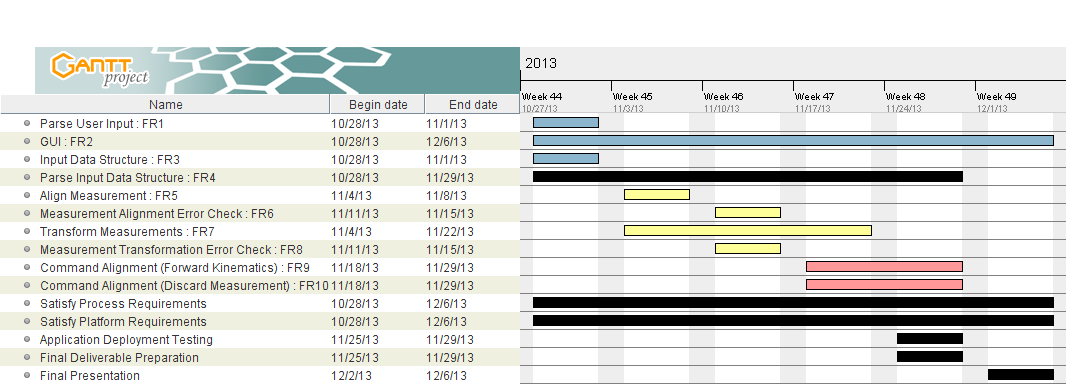
\includegraphics[width=185mm, height=61mm]{gantt.png}
\end{adjustwidth}
\end{center}

\newpage

\section*{Functional Requirements}
\begin{description}

\item[] FR1: Parse raw short tool and long tool CSV measurement, tool length, tool offset, and command position data into data structures. \newline [Developers: Charles Ortman | Time: 5 hours ]
\begin{enumerate}
\item The most optimal data structures will be determined to store the tool measurement, length, offset, and command position data for processing. [Time: 0.5 hours]
\item A class will be created with the data structures determined in Step 1 as private fields with basic get/set functionality. [Time: 1.0 hours]
\item Functions will be written for the input storage class that can parse the raw CSV format of the input files and GUI class input to store in the private fields. [Time: 3.5 hours]
\end{enumerate}

\item[] FR2: Provide GUI for selecting a machine configuration. \newline [Developers: Charles Ortman | Time: 5 hours ]
\begin{enumerate}
\item A graphic outline will be drafted on paper to map out the intended look of the machine configuration GUI. [Time: 0.5 hours]
\item A class will be coded that utilizes the WinForms .Net API to have the functionality to implement the appearance of the rough draft from Step 1. [Time: 3.0 hours]
\item Multiple functions will be written to associate calls from the GUI (including button presses and text input) with get/set functions from the input storage class. [Time: 1.0 hours]
\item The appearance of the functioning GUI will analyzed and refined to present an interface that achieves a definitive feel of elegance, usability, and professionalism. [Time: 0.5 hours]
\end{enumerate}

\item[] FR3: Indicate progress / current step of the application through the GUI. \newline [Developers: Charles Ortman | Time: 5 hours ]
\begin{enumerate}
\item A graphic outline will be drafted on paper to map out the intended look of the process tracking GUI. [Time: 0.5 hours]
\item The class written for the machine configuration GUI will be updated with any necessary functionality from the WinForms .Net API to implement the additional graphical needs determined in Step 1. [Time: 3.0 hours]
\item Multiple functions will be written to accept calls from other classes to indicate the progress of other processes in program. These functions will then in turn call the added functionality from Step 2 to display this progress. [Time: 1.0 hours]
\item The functioning process tracking GUI will be refined to be consistent with the appearance of the machine configuration GUI. [Time: 0.5 hours]
\end{enumerate}

\item[] FR4: Parse the input data structure to obtain inputs for each stage of the application. \newline [Developers: All | Time: Ongoing ]
\begin{enumerate}
\item All modules of the application will access the same data structures for communication.
\end{enumerate}

\item[] FR5: If the offset between long and short tool measurements is greater than two to three standard deviations, then attempt to align that offset or remove the measurement.
\newline [Developers: Alex Bertels | Time: 4 hours ]
\begin{enumerate}
\item Parse the long and short measurements data file. [Time: 0.5 hours]
\item Determine if the offset between the long and short tool measurements is greater than two to three standard deviations or greater than some maximum constant. [Time: 1.5 hours]
\item Attempt to align incorrect offsets or remove unmatched measurements using a brute force technique. [Time: 2 hours]
\end{enumerate}

\item[] FR6: If an offset cannot be aligned or too many measurements were not aligned, then throw an error asking for more or new long and short tool measurement data.
\newline [Developers: Alex Bertels | Time: 3 hours ]
\begin{enumerate}
\item Decide if an offset cannot be aligned or too many measurements were not aligned. [Time: 1.5 hours]
\item If there is a problem, throw an error asking for more or new long and short tool measurement data. [Time: 1.5 hours]
\end{enumerate}

\item[] FR7: Using the aligned measurements, parse the Calculate Transformation MATLAB DLL.
\newline [Developers: Alex Bertels | Time: 8 hours ]
\begin{enumerate}
\item Establish an environment to run MATLAB DLLs. [Time: 1.5 hours]
\item Convert the MATLAB script into a DLL capable of transforming measurements. [Time: 2.5 hours]
\item Using a C\# program, pass input to, execute, and read output from the MATLAB DLL automatically. [Time: 4 hours]
\end{enumerate}

\item[] FR8: If the transformation is deemed incorrect, assume that more or new long and short tool measurements are needed and throw an error stating so.
\newline [Developers: Alex Bertels | Time: 2 hours ]
\begin{enumerate}
\item Decide if the transformation was incorrect. [Time: 1.5 hours]
\item If there is a problem, throw an error asking for more or new long and short tool measurement data. [Time: 0.5 hours]
\end{enumerate}

\item[] FR9: Using forward kinematics, align commands such that for a predicted measured position of the machine for a given command, the actual measurement is close to the predicted value. \newline [Developers: Kevin Zheng | Time: 5 hours ]
\begin{enumerate}
\item Parse output from the transformed measurements data structure. [Time:.5 hours]
\item Load the machine forward kinematic from the data structure. [Time:.5 hours]
\item For each measurement in the aligned and transformed measurement, test that a predicted measurement value is reasonably close to a predicted value for that measurement. [Time: 4 hours]
\end{enumerate}

\item[] FR10: If an estimated command position and actual command position do not match, discard the measurement. The error should not be greater than $10^{-2}$.
\newline [Developers: Kevin Zheng | Time: 5 hours ]
\begin{enumerate}
\item Discard a command or measurement for all misaligned commands such that the actual and predicted values are close for every measurement in the data structure. [Time: 4 hours]
\item Continue attempting to align predicted values from commands to actual values from the transformed measurements tool. [Time: 1 hours]
\end{enumerate}

\item[] FR11: Parse controller profile to the GA Table Selection.
\newline [Developers: Kevin Zheng | Time: 1 hours ]
\begin{enumerate}
\item Read in the controller profile, based on user input, to a data structure containing arguments to the GA. [Time: 1 hour]
\end{enumerate}

\item[] FR12: Supply the aligned commands to the Implicit Loop Method and GA Table Selection MATLAB DLLs to obtain output for generating the tables and reports.
\newline [Developers: Kevin Zheng | Time: 4 hours ]
\begin{enumerate}
\item Open a handler for dynamically linked libraries and supply aligned data, tool lengths, relevant link lengths, and transformation from measurement frame to the ILM DLL. [Time: 1.5 hours]
\item Open a handler for dynamically linked libraries and supply aligned data, tool lengths, relevant link lengths, and transformation from measurement frame to the GA DLL. [Time: 1.5 hours]
\item Write all input and output to the ILM and GA to a data structure. [Time: 1 hours]
\end{enumerate}

\item[] FR13: Build performance report from the output of the Implicit Loop Method DLL containing a goodness of fit value, calculation time, mean and maximum residual error, and plots of the identified table function.
\newline [Developers: Joseph Steurer | Time: 6 hours ]
\begin{enumerate}
\item Parse output of ILM DLL into a data structure. [Time 1.5 hours]
\item Title and format the report in Microsoft Word format using a C\# library. [Time 1 hour]
\item Write the goodness of t value, calculation time, and mean and maximum residual error to a Microsoft Word document using a C\# library. [Time 1.5 hours]
\item Plot the identified table functions using a C\# library and output to the same document. [Time 2 hours]
\item Save the report to a directory. [Time 1 hour]
\end{enumerate}

\item[] FR14: Generate a second performance report from the output of the GA Tables DLL showing the solutions to the genetic algorithm, graph of errors, performance statistics, calculation time, chi squared value, and max/mean residual error.
\newline [Developers: Joseph Steurer | Time: 7.5 hours ]
\begin{enumerate}
\item Parse output of GA Tables DLL into a data structure. [Time: 1.5 hours]
\item Title and format the report in Microsoft Word format using a C\# library. [Time: .5 hours]
\item Write the performance statistics, calculation time, chi squared value and mean and maximum residual error to a Microsoft Word document using a C\# library. [Time 1.5 hours]
\item Plot the graph of errors using a C\# library and output to the same document. [Time: 2 hours]
\item Output the solutions to the genetic algorithm using a C\# library to the same document. [Time: 2 hours]
\end{enumerate}

\item[] FR15: Format the compensation tables populated by the GA algorithm based on a user specified controller type.
\newline [Developers: Joseph Steurer | Time: 3.5 hours ]
\begin{enumerate}
\item Open a file handler to begin parsing the raw tables generated from the GA. [Time .5 hours]
\item Select the controller based on user input. [Time .5 hours]
\item Format the tables according to a predefined controller specification. [Time 2 hours]
\item Save the formatted tables to a new file. [Time .5 hours]
\end{enumerate}
\end{description}

\section*{Quality Requirements}
\begin{description}
\item[] QR1: Integrate a manual discussing how the application transforms its input into output.
\newline [Developers: Joseph Steurer | Time: 6 hours ]
\begin{enumerate}
\item Identify the steps required to transform user input to output. [Time 1 hour]
\item Summarize the steps required to transform user input to output. [Time 2 hours]
\item Add a menu option to the user UI for accessing the manual. [Time .5 hours]
\item Show the steps neatly in a new window such that the user can understand how the application behaves. [Time 2.5 hours]
\end{enumerate}
\end{description}

\section*{Platform Requirements}
\begin{description}
\item[] PR1: Windows XP and Windows 7
\begin{enumerate}
\item Ensure the software runs on a Windows XP and Windows 7 platform.
\item Note missing dependencies such as libraries or .net framework installations.
\end{enumerate}
\item[] PR2: C\# / Microsoft Visual Studio
\begin{enumerate}
\item Obtain Visual Studio, write code using C\# .net.
\end{enumerate}
\item[] PR3: Mechanism for parsing output from the MATLAB DLL files.
\begin{enumerate}
\item Identify a C\# mechanism for parsing DLLs.
\item Ensure that input to a DLL and output from a DLL can be written from and read into the application’s memory.
\end{enumerate}
\item[] PR4: Library for interaction with compiled MATLAB code.
\begin{enumerate}
\item Obtain a library from mathworks to facilitate communication between C\# .net and compiled matlab code.
\item Add the library to the project.
\end{enumerate}
\item[] PR5: Library to support interaction with Microsoft Office for automatic report generation.
\begin{enumerate}
\item Obtain a library for generating Microsoft Word documents using C\#.
\item Add the library to the project.
\end{enumerate}
\item[] PR6: Library to generate plots based on data obtained from MATLAB DLL.
\begin{enumerate}
\item Obtain a library for generating plots using C\#.
\item Add the library to the project.
\end{enumerate}
\end{description}

\section*{Process Requirements}
\begin{description}
\item[] The development group must provide weekly or bi-weekly updates to clients.
\begin{enumerate}
\item Set up meetings with Boeing contacts.
\item Establish agenda for team meetings.
\item Provide feedback, answer questions, explain progress and goals.
\end{enumerate}
\item[] Coding will be managed in sprints, where the team meets to code as a group.
\begin{enumerate}
\item Team will meet in a classroom to work on project coding.
\item The team will work off of individual laptops.
\end{enumerate}
\item[] Develop test cases for each step of the application to verify the correctness of output at the end of each processing step.
\begin{enumerate}
\item Consider possible ways to break a requirement.
\item Add test cases for these considerations.
\item Resolve errors and document results of test.
\end{enumerate}
\item[] Version control must be employed throughout the development process.
\begin{enumerate}
\item Use the Git versioning system.
\item Team members will push and pull from the same repository.
\item Each team member has his own branch.
\item Team Lead will merge team member branches into master.
\end{enumerate}
\end{description}

\end{document}



